\subsection{Présentation de la problématique}
 
Dans certains systèmes IoT, les données qui sont utilisées ont une importance cruciale, voire vitale. Ces données se doivent être fiables, et disponibles. Dans le domaine du Smart Health, où les capteurs sont utilisés pour surveiller des indices vitaux du patient, leur dysfonctionnement pourrait mettre en péril la vie du patient en envoyant des données erronées qui peuvent induire le personnel médical en erreur. Les systèmes utilisés dans l’IoT peuvent comprendre des actionneurs ou agir sur des objets, qui eux vont avoir des répercussions sur une éventuelle personne. C’est pourquoi l’utilisation de ces objets doit être fiables.

Dans notre système pour la surveillance des patients dans le département des soins intensifs, les problématiques de fiabilité, de tolérance aux pannes et de disponibilité ont une importance cruciale car elles ont un lien avec la vie du patient. La fiabilité des dispositifs qui sont proposés dans le domaine de la santé doit être capable de détecter immédiatement toute défaillance ou panne d’un objet pour que des mesures puissent être prises en conséquence. Notre architecture en couches permet de repérer une éventuelle défaillance ou une panne d’un dispositif. Les données et actionneurs dans notre système doivent être disponibles pour le personnel médical qui pourra l’utiliser pour s’aider dans ses tâches quotidiennes. Les problématiques que nous voyons dans notre système sont liées aux problématiques de sécurité. Nous verrons dans la suite de cette section les mesures que nous avons prises pour s’assurer d’un minimum de QoS dans notre architecture à travers les différentes couches.

\subsection{Prise en compte de cette problématique dans la couche physique}

Les problématiques de QoS se retrouvant dans toute l’architecture que nous avons proposée, nous les avons prises en compte dans chacune des couches. Notre solution détaillée dans les différents rapports comprend un grand nombre d’éléments répondant à ces objectifs que nous allons récapituler ici.

Dans la couche physique, une première mesure afin d’améliorer la disponibilité pour permettre aux médecins d’être notifiés rapidement en cas de variations anormales, est de connecter les moniteurs via Ethernet au réseau de l’hôpital. Cela permet une plus grande capacité et limite le nombre d’interférences liées aux ondes. Une telle méthode permettrait de ne pas causer de dysfonctionnement avec d’autres appareils sensibles comme un scanner.

Au niveau de la couche de communication, notre système utilise le protocole UDP (avec sa sur-couche DTLS) pour l’envoi de données fréquentes au Smart Gateway depuis le moniteur. Par données fréquentes, nous entendons des données qui sont fréquemment mises à jour. Pour de telles données, la perte de quelques paquets de manière épisodique n’est pas pénalisante, car elles sont mises à jour régulièrement. Un mécanisme applicatif détectera les pertes consécutives et déclenchera des avertissements afin qu’un membre du personnel de l’hôpital aille vérifier l’état du capteur concerné. En revanche, pour les mesures prises de façon plus rares, un mécanisme d’accusé de réception est présent afin de ne pas perdre de données.

Pour la fiabilité et la disponibilité des dispositifs, dès qu’une mesure anormale est détectée, il faut connaître la raison de cette anomalie. Si elle provient de l’appareil, une alerte sera déclenchée. Pour cela, on pourrait s’appuyer sur la fabrication d’un appareil qui intégrera certains cas de défaillance, ce qui nous permettra d’avertir un technicien, qui pourra être envoyé pour vérifier les capteurs pour des valeurs non conformes. Pour les autres anomalies détectées, un membre du personnel médical sera envoyé sur place. Ce sera à lui de vérifier que les données sont bien reliées au patient et non a une erreur du dispositif, et d’appeler un technicien le cas échéant.

Un timeout est présent pour la détection de pannes afin de lancer une alerte en l’absence de données durant un certain laps de temps. Selon les informations que caractérisent ces données, l’alerte ne sera pas la même. En effet, le dysfonctionnement d’un capteur selon ce qu’il mesure (fréquence cardiaque, température de la salle) n’a pas le même impact. Le signal envoyé (alerte, avertissement, notification) est en fonction de la gravité de la panne afin que les pannes les plus graves soient traitées en premier. Cette hiérarchisation est rappelé sur la figure \ref{alerte}.
\newline
\begin{figure}[h!]
	\hspace*{-2.5cm}
	\centering
	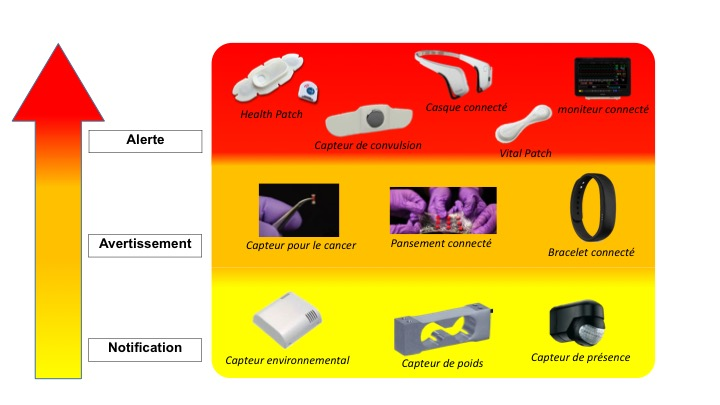
\includegraphics[width=1.4\textwidth]{alerte.jpg}
	\caption{Hiérarchisation des Signaux de Dysfonctionnement en fonction des Dispositifs}
	\label{alerte}
\end{figure}


\subsection{Prise en compte de ces problématiques dans le middleware}
 
La fiabilité d’un middleware est une exigence essentielle. Un middleware doit rester opérationnel pendant toute la durée d’une mission, même en présence de pannes. La fiabilité du middleware fait partie intégrante de la réalisation de la fiabilité au niveau du système. Chaque composant ou service dans un middleware doit être fiable pour atteindre la fiabilité globale, ce qui inclut celles de la communication, des données, des technologies et des dispositifs de toutes les couches. Les signes vitaux qui sont surveillés imposent au middleware d’être capable de transmettre les données de façon fiable sans corruption de celles-ci, à cause des données qui sont surveillées.

En cas de défaillance de notre système, le temps de récupération et la fréquence de défaillance de celui-ci sont suffisamment petits pour obtenir la disponibilité souhaitée. Les exigences en matière de fiabilité et de disponibilité doivent travailler ensemble pour assurer la plus haute tolérance aux pannes nécessaire depuis une application. Les middlewares de notre système peuvent détecter si l’un de nos capteurs est en panne, et pour cela, il va faire des requêtes à intervalles réguliers des signes vitaux, et en cas d’absence de réponse pendant un temps prédéfini, une alerte sera envoyée au personnel médical pour vérifier l’origine de l’erreur. Dans le domaine de la santé, où la vie des patients est en jeu, nous ne pouvons pas nous permettre de laisser le patient sans surveillance médicale.

Un module de détection des pannes est présent dans les différents middlewares. En effet, de par l’importance des données fournies par ces capteurs, il faut les remplacer dès le premier indice de dysfonctionnement. De manière générale, il est important de garantir une bonne disponibilité ainsi qu’une certaine fiabilité. Ces considérations sur la détection de pannes imposent de disposer d’un module d’émission d’évènements afin que le middleware du moniteur intelligent puisse avertir immédiatement la Smart Gateway d’un dysfonctionnement d’un capteur, ou d’une valeur anormale par rapport au profil du patient (par exemple une crise cardiaque).

\subsection{Prise en compte vis-à-vis des applications}
 
Les applications que nous proposons ont pour but d’être utilisées sur des téléphones intelligents, des tablettes ou des ordinateurs. Dans le cadre de notre architecture, les applications sur lesquelles la QoS est importante sont celles liées au personnel médical.

Nous avons décrit différents processus pour assurer un minimum de QoS dans les couches précédentes, nous allons nous intéresser maintenant à comment les données vont être récupérées et utilisées. Dans ce qui a été décrit au niveau des applications, celles-ci nous permettent de centraliser les différentes données des différents capteurs. Ces données peuvent être récupérées directement à partir des capteurs ou depuis le système de stockage pour la consultation d’historique.

Les détections d’anomalies sont mises en place au niveau du Gateway et qui font remonter à l’application les différentes pannes détectées. Les applications vont pouvoir agir sur les seuils de détections d’anomalies pour que le personnel médical puisse ajuster en fonction du profil du patient les différents capteurs. Les applications utilisées par le personnel médical vont principalement être utilisées pour avertir le personnel médical de différentes alertes et anomalies provenant des différents dispositifs. Au niveau de l’application utilisée pour la consultation plus détaillée d’un profil d’un patient, l’utilisateur sera notifié des différentes alertes qui lui sont destinées pour qu’il puisse les prendre en charge avec la possibilité d’informer le système de sa non-disponibilité. Les différentes alertes vont être aussi affichées sur l’application centrale, pour une redondance des informations et pour que l’alerte soit au moins visible par l’équipe médical d’astreinte en cas de défaillance d’un dispositif d’un membre du personnel médical.

La détection des pannes matérielles se fera au niveau du middleware et de la smart Gateway qui feront remonter l’information au niveau de l’application centrale pour qu’un membre du personnel médical puisse se diriger sur la zone de la panne et prendre les mesures adéquates.

Au niveau de la disponibilité des données, le système de stockage interne à l’hôpital va permettre aux différentes applications de chercher les informations dans le réseau local et de ne pas être dépendant d’Internet.  Ce qui rendra disponible les différentes données en tout temps sauf en cas de rupture complet du réseau interne, qui est un cas qui devra être relativement rare.

Enfin la fiabilité des données qui transitent dans notre réseau va essentiellement reposer sur la fiabilité des dispositifs qui vont être présents dans notre système. Ces dispositifs seront choisis en fonction de la réputation du constructeur et de la qualité des capteurs. Outre des problèmes au niveau des capteurs, notre réseau ne devrait pas, avec les mesures de sécurité proposées, altérer les données transmises par les capteurs.      
